%18/11 - Dido Carrero
\part{Variantes genómicas: técnicas, llamada de variantes y anotación}
\chapter{Introducción a las variantes germinales}
\section{Análisis genómico}
El análisis genómico incluye varios pasos: primero, la extracción de muestras y la preparación de las librerías; luego, la secuenciación, el control de calidad de los archivos FastQ (donde se descartan las lecturas con errores, ya que una mayor refinación del pipeline implica un control de calidad más estricto); el alineamiento de las lecturas; la identificación o llamada de variantes (SNP, INDEL, CNV, SV); la anotación de los archivos VCF; la visualización de las variantes candidatas y, finalmente, los pasos de priorización y filtrado.

En general, en un análisis de genoma, pueden encontrarse muchas variantes en comparación con el genoma de referencia, por lo que es necesario aplicar filtros para identificar aquellas que sean realmente relevantes a nivel clínico. La validación final se realiza en el laboratorio mediante PCR.

Las variantes germinales se originan en la línea germinal, es decir, en los gametos, lo que las hace heredables y presentes en todo el organismo. En cambio, las variantes somáticas ocurren en células que no pertenecen a los gametos, son mutaciones adquiridas durante la vida y afectan solo a un linaje celular específico.

En la práctica, ya sea que se realice un análisis somático o germinal, se extraen muestras tanto del tejido tumoral como del tejido sano. Si se sospecha de una enfermedad genética germinal, también se debe extraer una muestra de un tejido germinal.

La frecuencia alélica es la proporción de moléculas de ADN en la muestra que contienen una mutación específica. Se calcula mediante la siguiente fórmula:
$$VAF = \frac{sequence.reads.with.a.DNA.variant}{overall.coverage.at.that.locus}$$
Este número es clave para diferenciar una variante somática de una germinal. En un organismo diploide, un locus heterocigoto debería mostrar un VAF cercano a 0,5, un locus homocigoto tendrá un VAF de 1 y un locus de referencia tendrá un VAF de 0. Las variantes somáticas presentan una frecuencia alélica muy variable, mientras que las variantes germinales suelen tener valores de VAF de 0, 0,5 o 1, dependiendo de si están presentes en uno, ambos o ninguno de los alelos.

\subsection{GATK}
GATK es un conjunto de herramientas desarrollado por el Broad Institute para el análisis de variantes genómicas. A partir de archivos BAM, estas herramientas permiten realizar un análisis completo de variantes. El paquete incluye buenas prácticas y un flujo de trabajo (workflow) que varía dependiendo de si se analizan variantes germinales o somáticas.

\begin{figure}[h!]
\centering
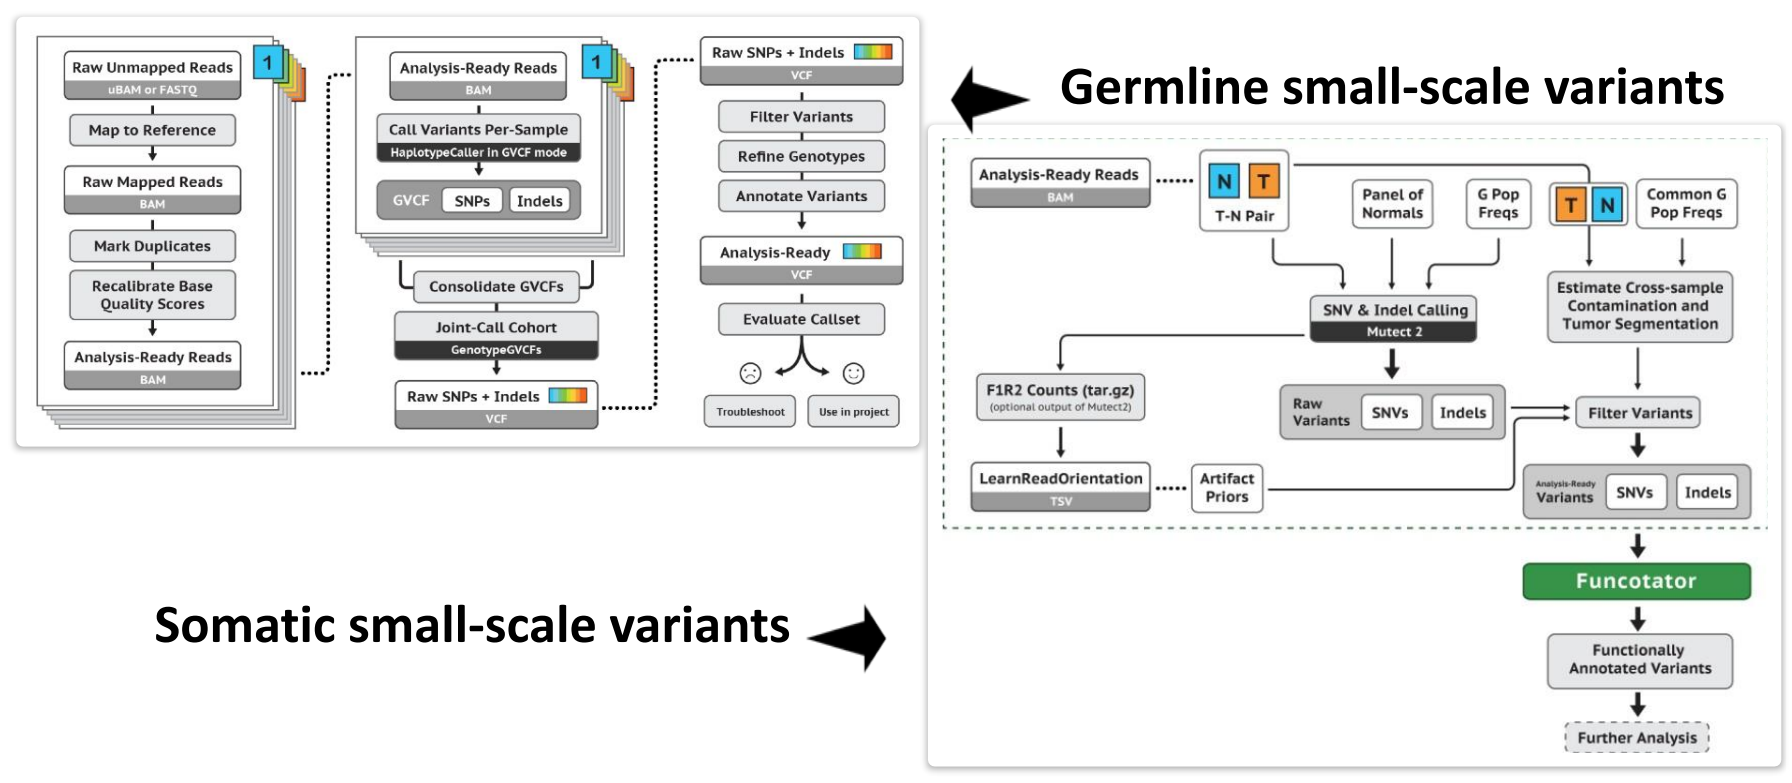
\includegraphics[width = 0.8\textwidth]{figs/gatk-pipelines.png}
\end{figure}

HaplotypeCaller es una herramienta utilizada para la llamada de variantes, basándose en el cálculo de la probabilidad de los genotipos. Utiliza un archivo BAM como entrada y produce un archivo de salida en formato VCF o GVCF con los genotipos 1/1, 0/1 y 0/0. Este archivo VCF debe ser filtrado mediante recalibración de bases (una práctica recomendada) o mediante hard-filtering. Si el archivo de salida es un GVCF, será necesario realizar un paso intermedio antes de aplicar el filtro y continuar con el análisis posterior. Además, con la opción -ploidy, se puede especificar la ploidía del organismo.

El comando básico para la herramienta es:
\begin{lstlisting}[language = bash]
gatk HaplotypeCaller \
	-R reference.fasta \
	-I preprocessed_reads.bam \
	-O germline_variants.vcf
\end{lstlisting}

MuTect2 es una herramienta diseñada para la llamada de variantes somáticas. Permite detectar SNVs e INDELs, con frecuencias alélicas variables, y es capaz de diferenciar entre variantes somáticas y germinales. MuTect2 ofrece varios modos: tumor con normal emparejado, solo tumor o modo mitocondrial.

\section{Práctica: análisis de datos}
Vamos a recibir los datos de cáncer de mama. Se ha secuenciado todo el exoma con Illumina. Primero creamos el entorno conda \texttt{OVCA\_case}. 
\begin{lstlisting}[language=bash]
conda create -n OVCA_case
conda activate OVCA_case
conda install bioconda::gatk4
conda install bioconda::samtools
\end{lstlisting}

Con los datos descargados, utilizamos la herramienta HaplotypeCaller. Lo primero que debemos hacer es realizar los índices de la referencia y del fichero bam:
\begin{lstlisting}[language=bash]
samtools dict  REFERENCE/hg19_chr17.fa -o  REFERENCE/hg19_chr17.dict
samtools faidx REFERENCE/hg19_chr17.fa
samtools index bams/normal_refined.bam
\end{lstlisting}

A continuación utilizamos la herramienta:
\begin{lstlisting}[language=bash]
gatk HaplotypeCaller -R REFERENCE/hg19_chr17.fa -I bams/normal_refined.bam -O out/normal_refined_out.vcf
\end{lstlisting}

El fichero resultante empieza con una cabecera con dos almohadillas y el cromosoma de referencia. Se muestra la información acerca de la generación del fichero y los filtros. Con una almohadilla se muestra el significado de cada columna: cromosoma en el que está la variante, posición genómica, ID, alelo de referencia, alelo alternativo con la mutación encontrada, score de calidad, filtros, información adicional con la anotación, formato del siguiente campo y normal. Dentro del formato, se distinguen: GT indica el genotipo, AD el número de lecturas que soporta la variante (en formato referencia,variante) y DP el total de lecturas.

El siguiente paso es la recalibración de variantes. Muchas veces, la calidad de las variantes que aparece de manera directa (columna QUAL) se debe recalibrar. Este modelo puntúa las calidades de las variantes y filtrar aquellas que no pasen los filtros. Se comprueba que una variante sea efectivamente verdadera. Para ello, se da un archivo de referencia de variantes y se estima si la variante es un artefacto de la secuenciación o una variante de verdad. El resultado es VQSLOD, que se añade al campo de información. Esto en general se realiza para SNPs e INDELs por separado debido a que las bases de datos de variantes son diferentes. 

El paso siguiente es aplicar los filtros VQSR. En la columna FILTER anota si la variante pasa filtros o no, pero no descarta aquellos que no pasen los filtros; si se quiere eso se debe especificar.
\begin{lstlisting}[language=bash]
tabix -p vcf Annotations/dbsnp_138.hg19_chr17.vcf.gz

gatk VariantRecalibrator -R REFERENCE/hg19_chr17.fa -V out/normal_refined_out.vcf
--resource:dbsnp,known=true,training=true,truth=true,prior=15.0
Annotations/dbsnp_138.hg19_chr17.vcf.gz -an QD -an ReadPosRankSum -an FS -an SOR -mode BOTH -O out/output_normal_refined.recal --tranches-file out/output_normal_refined.tranches

gatk ApplyVQSR -R REFERENCE/hg19_chr17.fa -V out/normal_refined_out.vcf -O out/output_normal_refined.recalibrated --truth-sensitivity-filter-level 99.0 --tranches-file out/output_normal_refined.tranches --recal-file out/output_normal_refined.recal -mode BOTH
\end{lstlisting}

El último paso es el filtrado de las variantes. 
\begin{lstlisting}[language=bash]
awk -F '\t' '{if ($0 ~ /#/ || $7 == "PASS") print}' out/output_normal_refined.recalibrated > out/output_normal_refined.onlypass

#Contar el número de líneas resultantes
grep "^chr17" out/output_normal_refined.onlypass | wc -l
\end{lstlisting}